\documentclass{beamer}
\usepackage[T1]{fontenc}
\usepackage[utf8]{inputenc}
\usepackage{lmodern}
\usepackage{amsmath}
\usepackage{amsfonts}
\usepackage{amssymb}
\usepackage{amsthm}
\usepackage{graphicx}
\usepackage{color}
\usepackage{xcolor}
\usepackage{url}
\usepackage{textcomp}
\usepackage{hyperref}
\usepackage{parskip}
\usepackage{algpseudocode}
\usetheme{CambridgeUS}
\makeatletter
\setbeamertemplate{footline}
{
  \leavevmode%
  \hbox{%
  \begin{beamercolorbox}[wd=.333333\paperwidth,ht=2.25ex,dp=1ex,center]{author in head/foot}%
    \usebeamerfont{author in head/foot}\insertshortauthor%~~\beamer@ifempty{\insertshortinstitute}{}{(\insertshortinstitute)}
  \end{beamercolorbox}%
  \begin{beamercolorbox}[wd=.333333\paperwidth,ht=2.25ex,dp=1ex,center]{title in head/foot}%
    \usebeamerfont{title in head/foot}\insertshorttitle
  \end{beamercolorbox}%
  \begin{beamercolorbox}[wd=.333333\paperwidth,ht=2.25ex,dp=1ex,right]{date in head/foot}%
    \usebeamerfont{date in head/foot}\insertshortdate{}\hspace*{2em}
    \insertframenumber{} / \inserttotalframenumber\hspace*{2ex} 
  \end{beamercolorbox}}%
  \vskip0pt%
}
\makeatother

\title{Opening CoViD Centers at Given Hospitals}
\subtitle{the k-center problem}
\author{Karamjot Kaur, Sudipto Ghosh}
\institute{\emph{M.Sc. CS Semester I\\Department of Computer Science\\University of Delhi}}
\date{\today}

\begin{document}

\begin{frame}
    \titlepage
\end{frame}

\begin{frame}
    \frametitle{Problem Definition}
    \begin{itemize}
        \item Find 4 locations to open the CoViD centers such that the maximum distance of any patient from the nearest CoViD facility is minimized.
        \item Locate a set of $k$ facilities given a set of demand nodes, such that, for any demand point, the nearest facility is as close is possible.
        \item Similar to clustering a set of data points and computing cluster centers, such that the intracluster distance is minimized.
    \end{itemize}
\end{frame}

\begin{frame}
    \frametitle{Problem Definition}
    Given a complete, undirected graph $G = (V, E)$ with distances on edges satisfying the triangle inequality, and a positive integer $k < |V|$.
    
    The problem is to find such a set $C \subset V$, where $|C| < k$, which minimizes the maximum distance from any node in $V$ to its closest center.
    
    Mathematically, minimize $\underset{v \in V}{\max}\;\underset{c \in C}{\min}\;d(v,c)$.
    
    A polynomial time solution to this problem is not known.
\end{frame}

\begin{frame}
    \frametitle{Verifiable?}
    We can just iterate over all data points or patients and check whether the distance from its assigned cluster center or their assigned CoViD center is located at most some non-negative integral distance $d$ away or not.
    
    This checking algorithm can indeed verify a certificate to the problem in polynomial time.
    
    Therefore, the CoViD center location problem is in NP.
\end{frame}

\begin{frame}[c]
    \frametitle{Dry Run}
    \centering 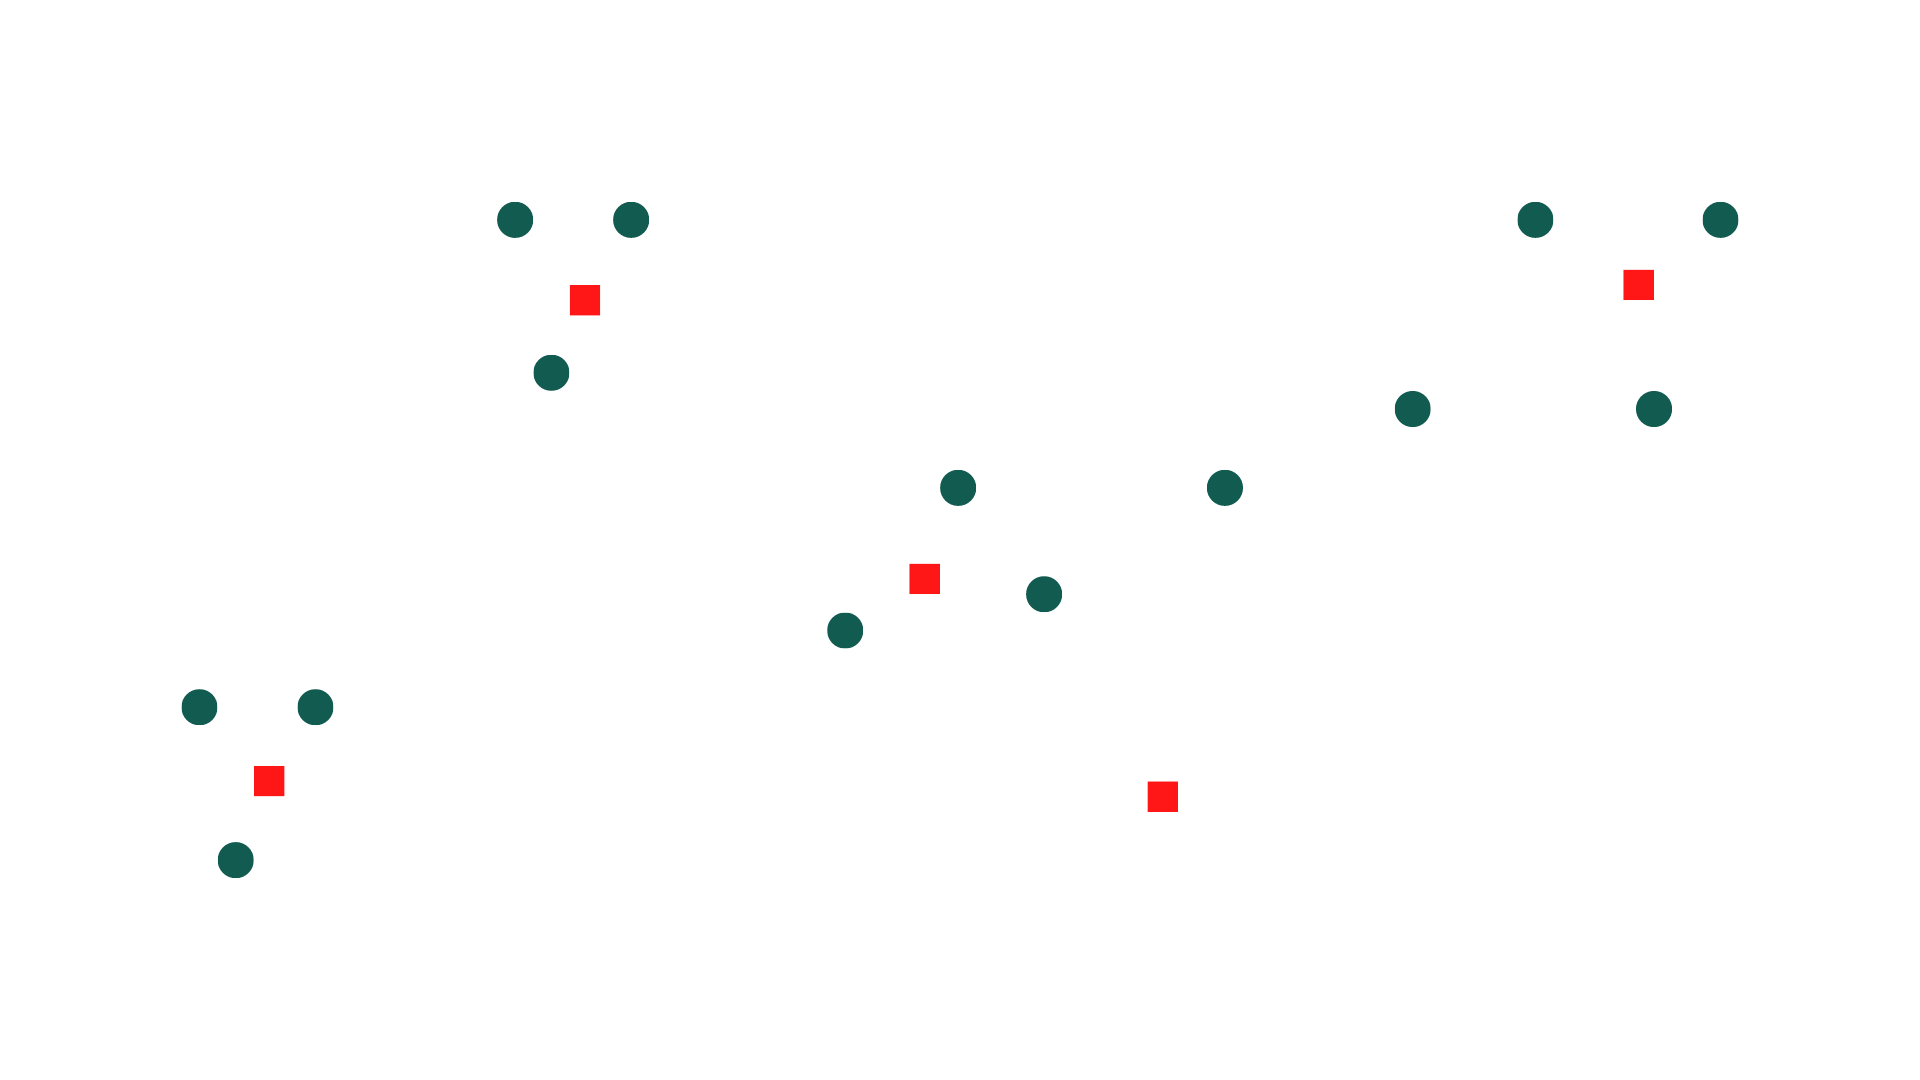
\includegraphics[width=350pt]{./5.png}
\end{frame}

\begin{frame}[c]
    \frametitle{Dry Run}
    \centering 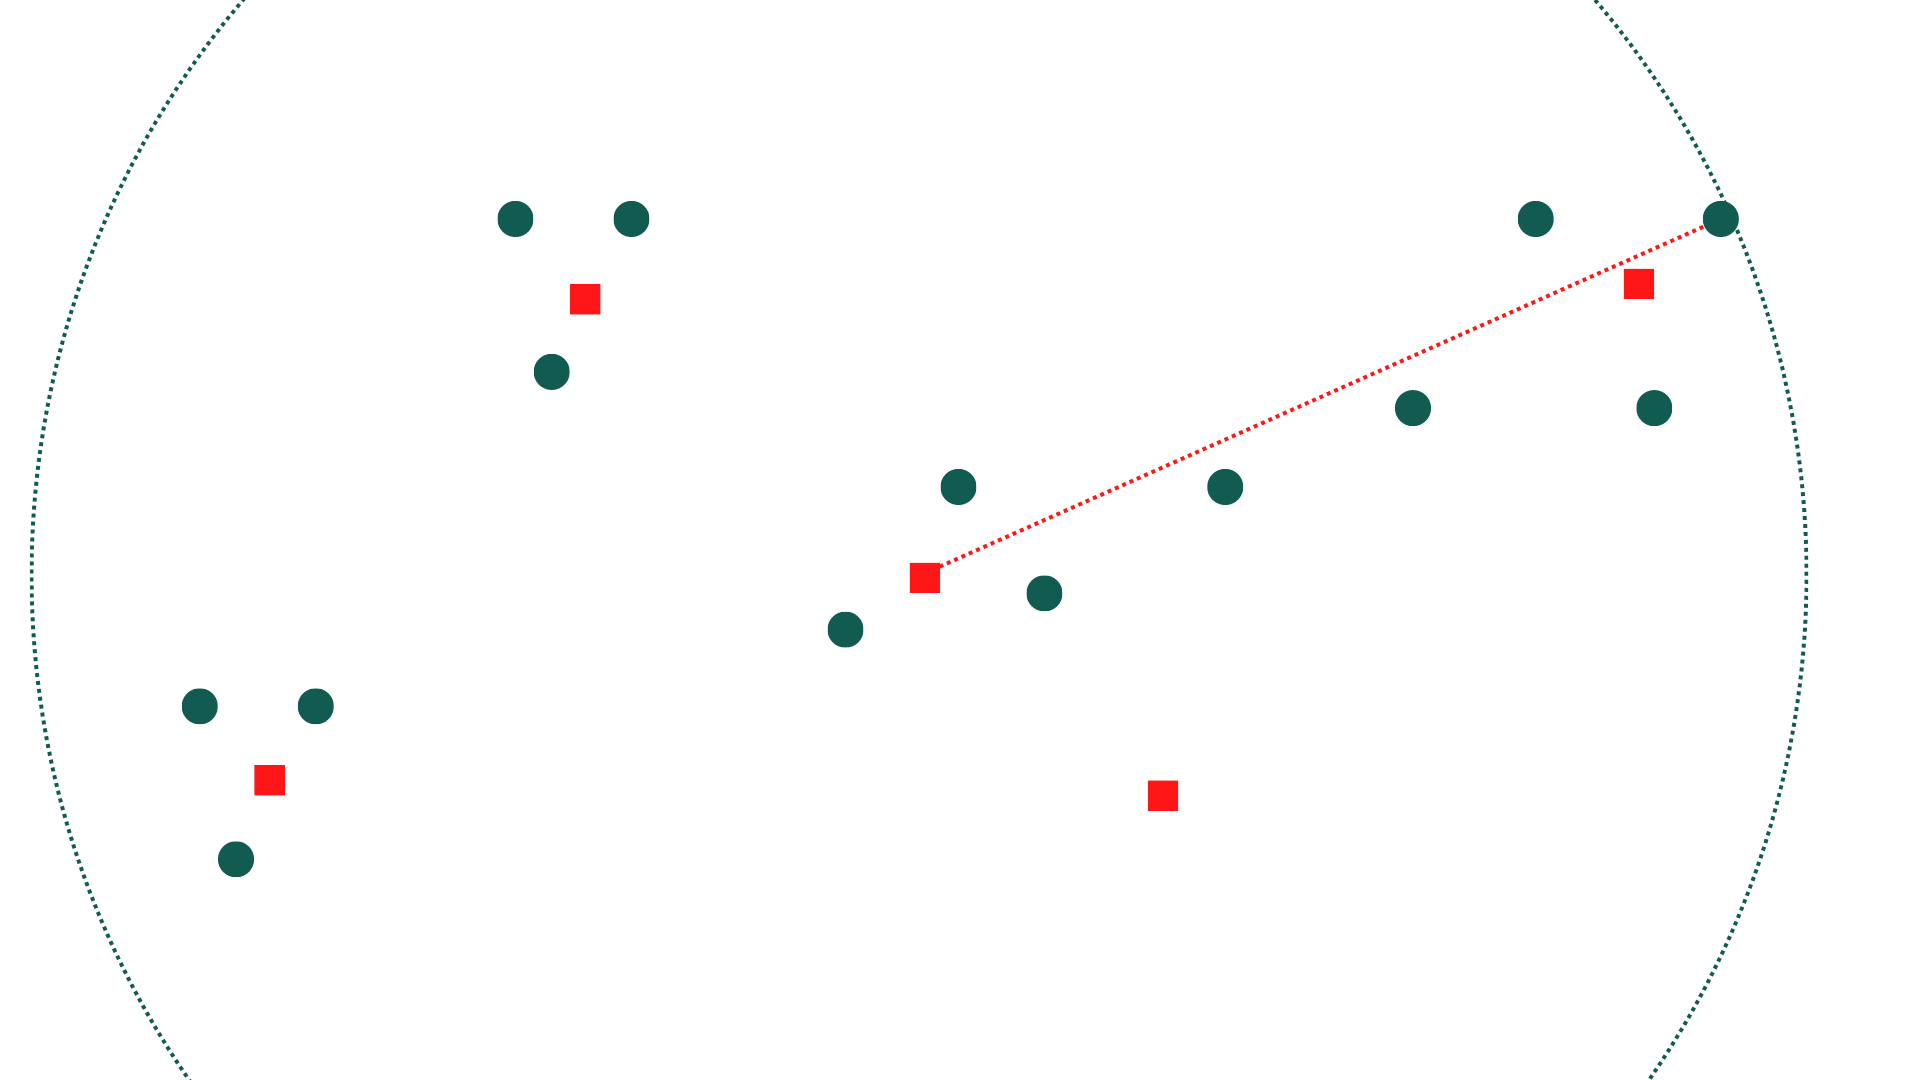
\includegraphics[width=350pt]{./6.png}
\end{frame}

\begin{frame}[c]
    \frametitle{Dry Run}
    \centering 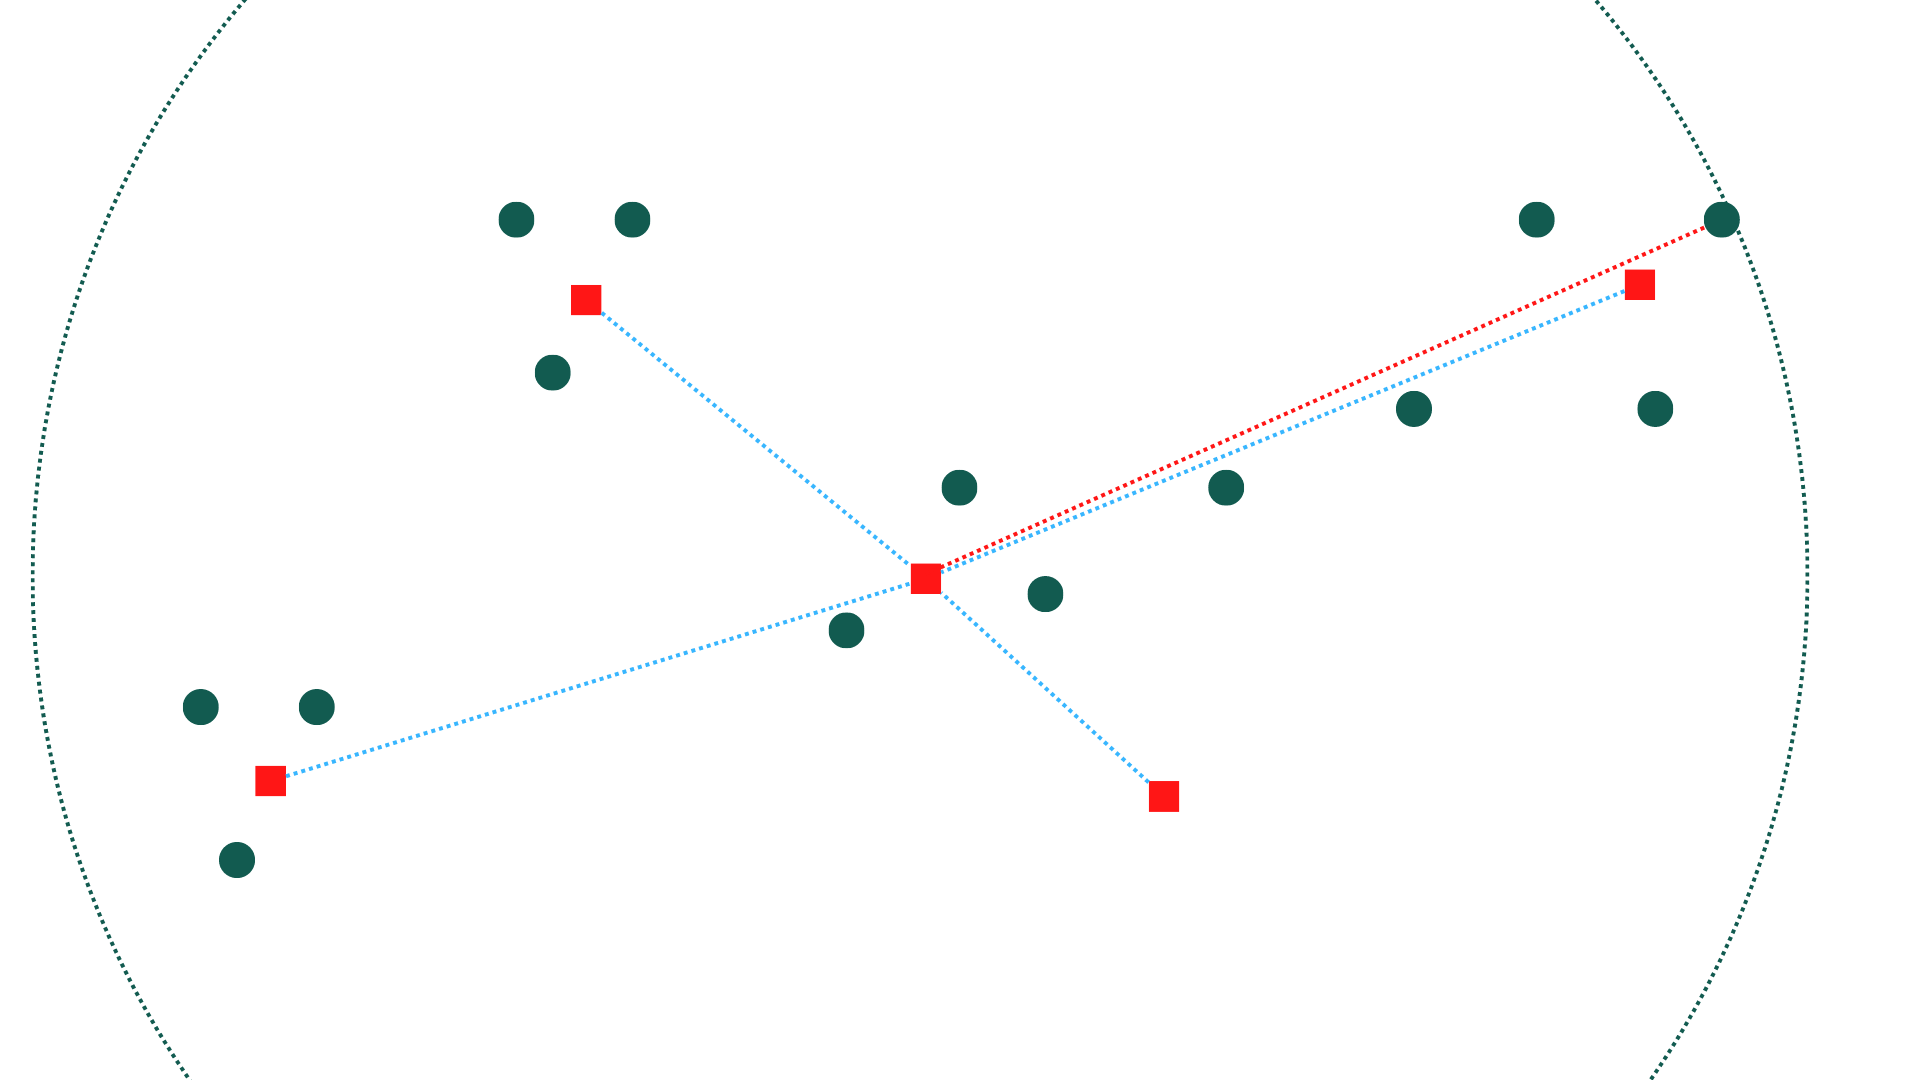
\includegraphics[width=350pt]{./7.png}
\end{frame}
   
\begin{frame}[c]
    \frametitle{Dry Run}
    \centering 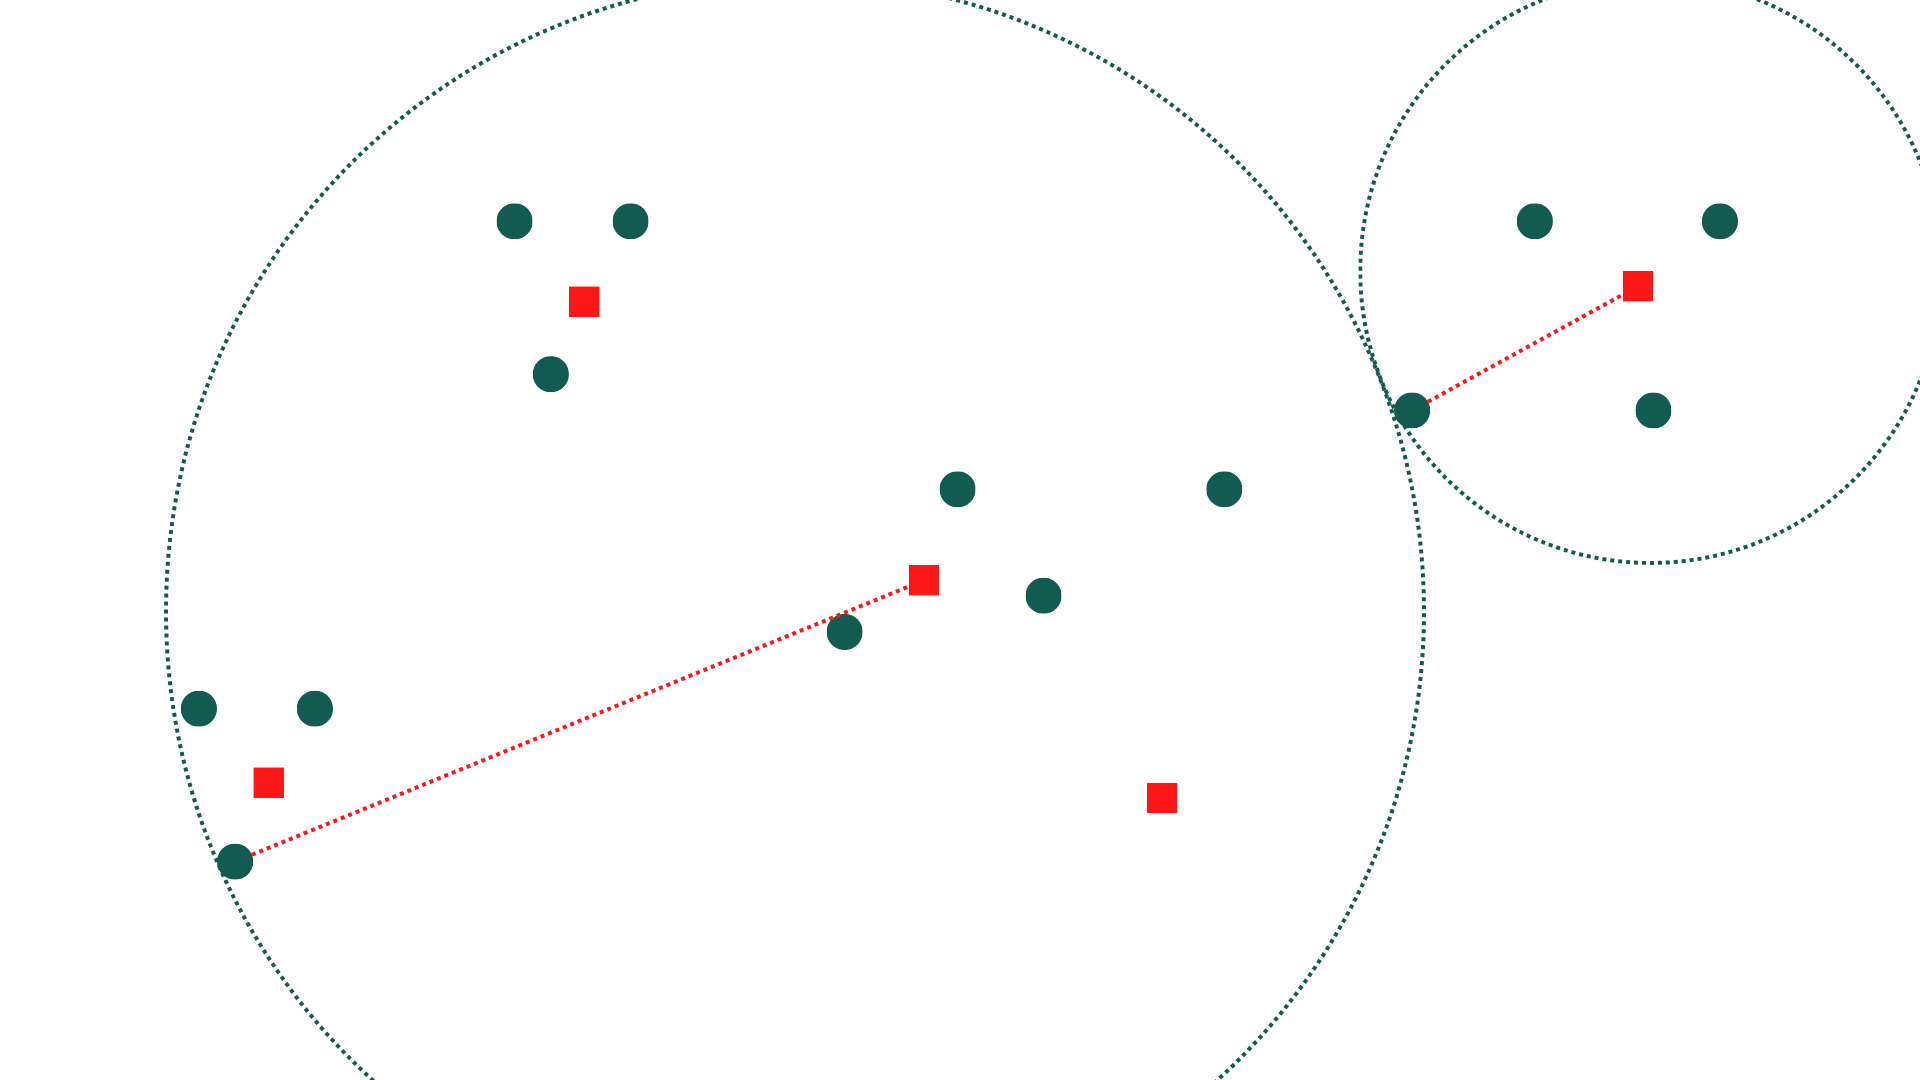
\includegraphics[width=350pt]{./8.png}
\end{frame}   

\begin{frame}[c]
    \frametitle{Dry Run}
    \centering 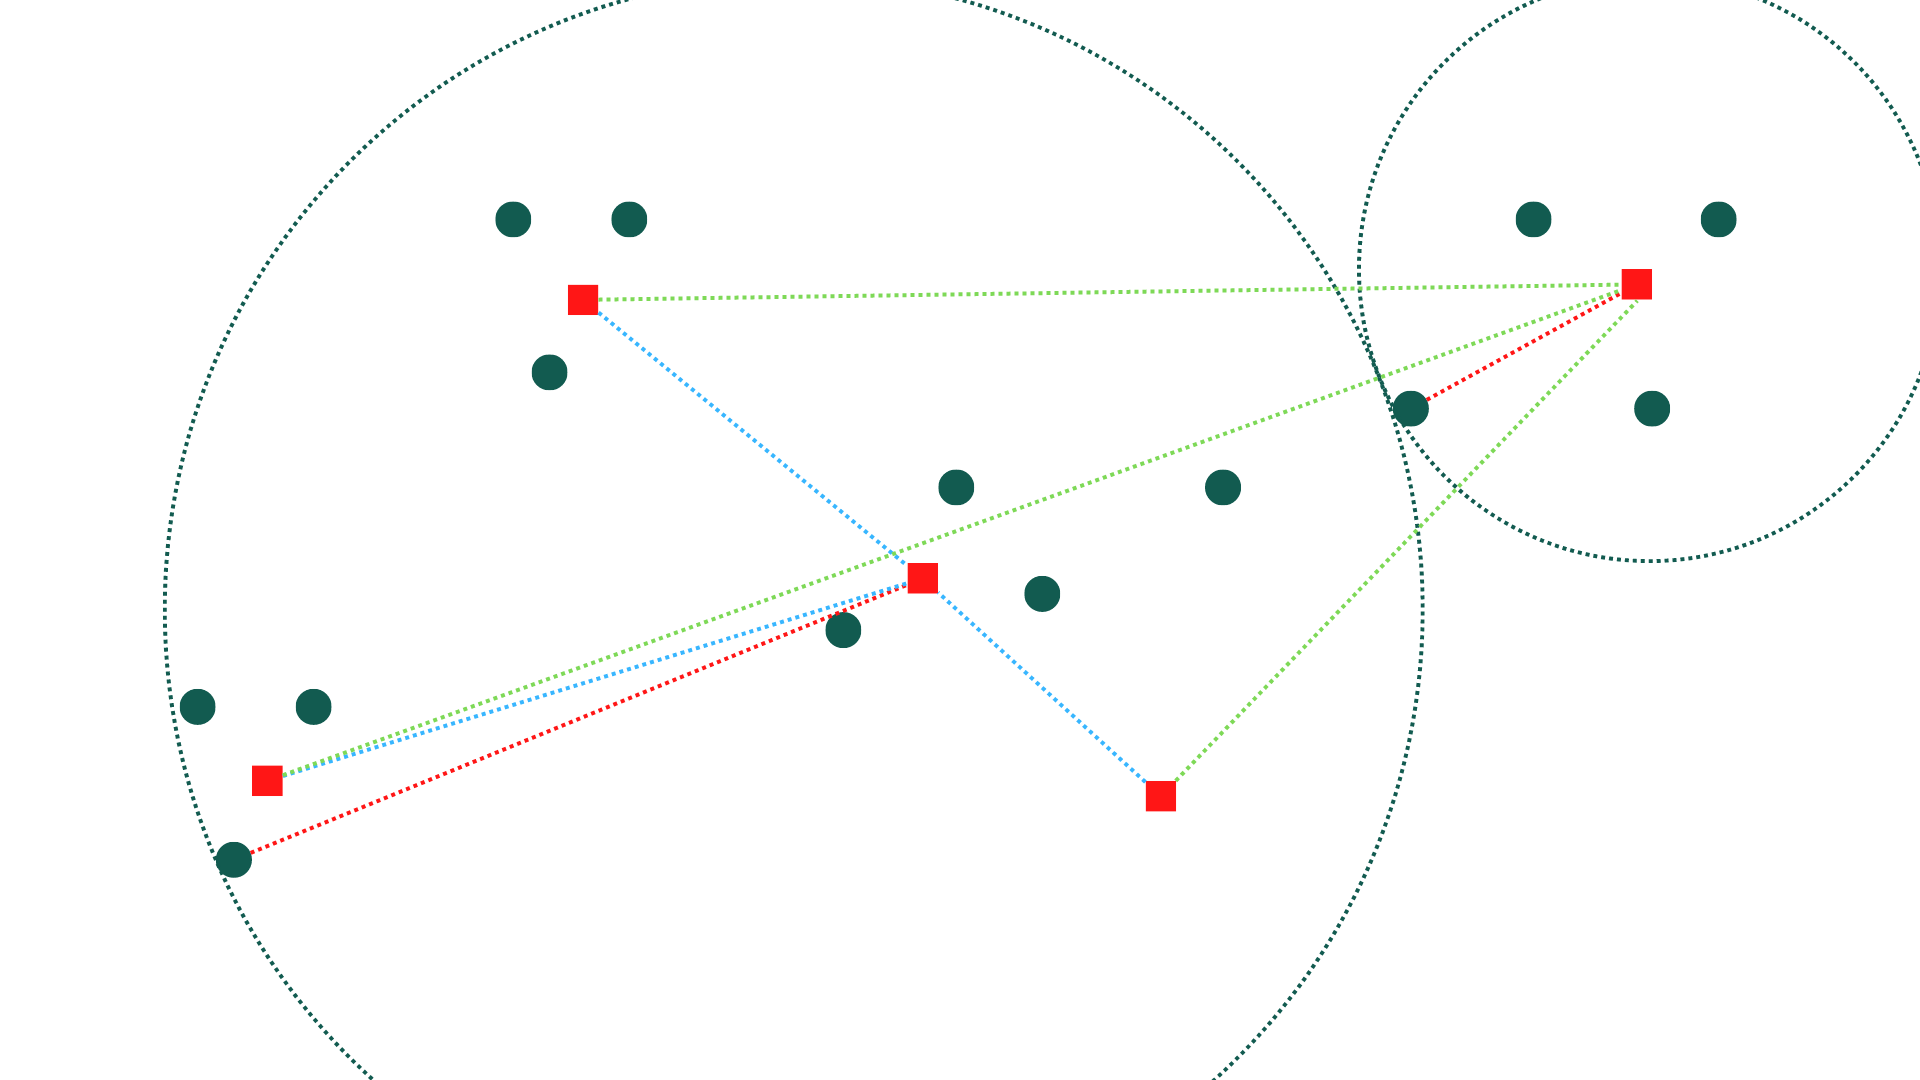
\includegraphics[width=350pt]{./9.png}
\end{frame}
   
\begin{frame}[c]
    \frametitle{Dry Run}
    \centering 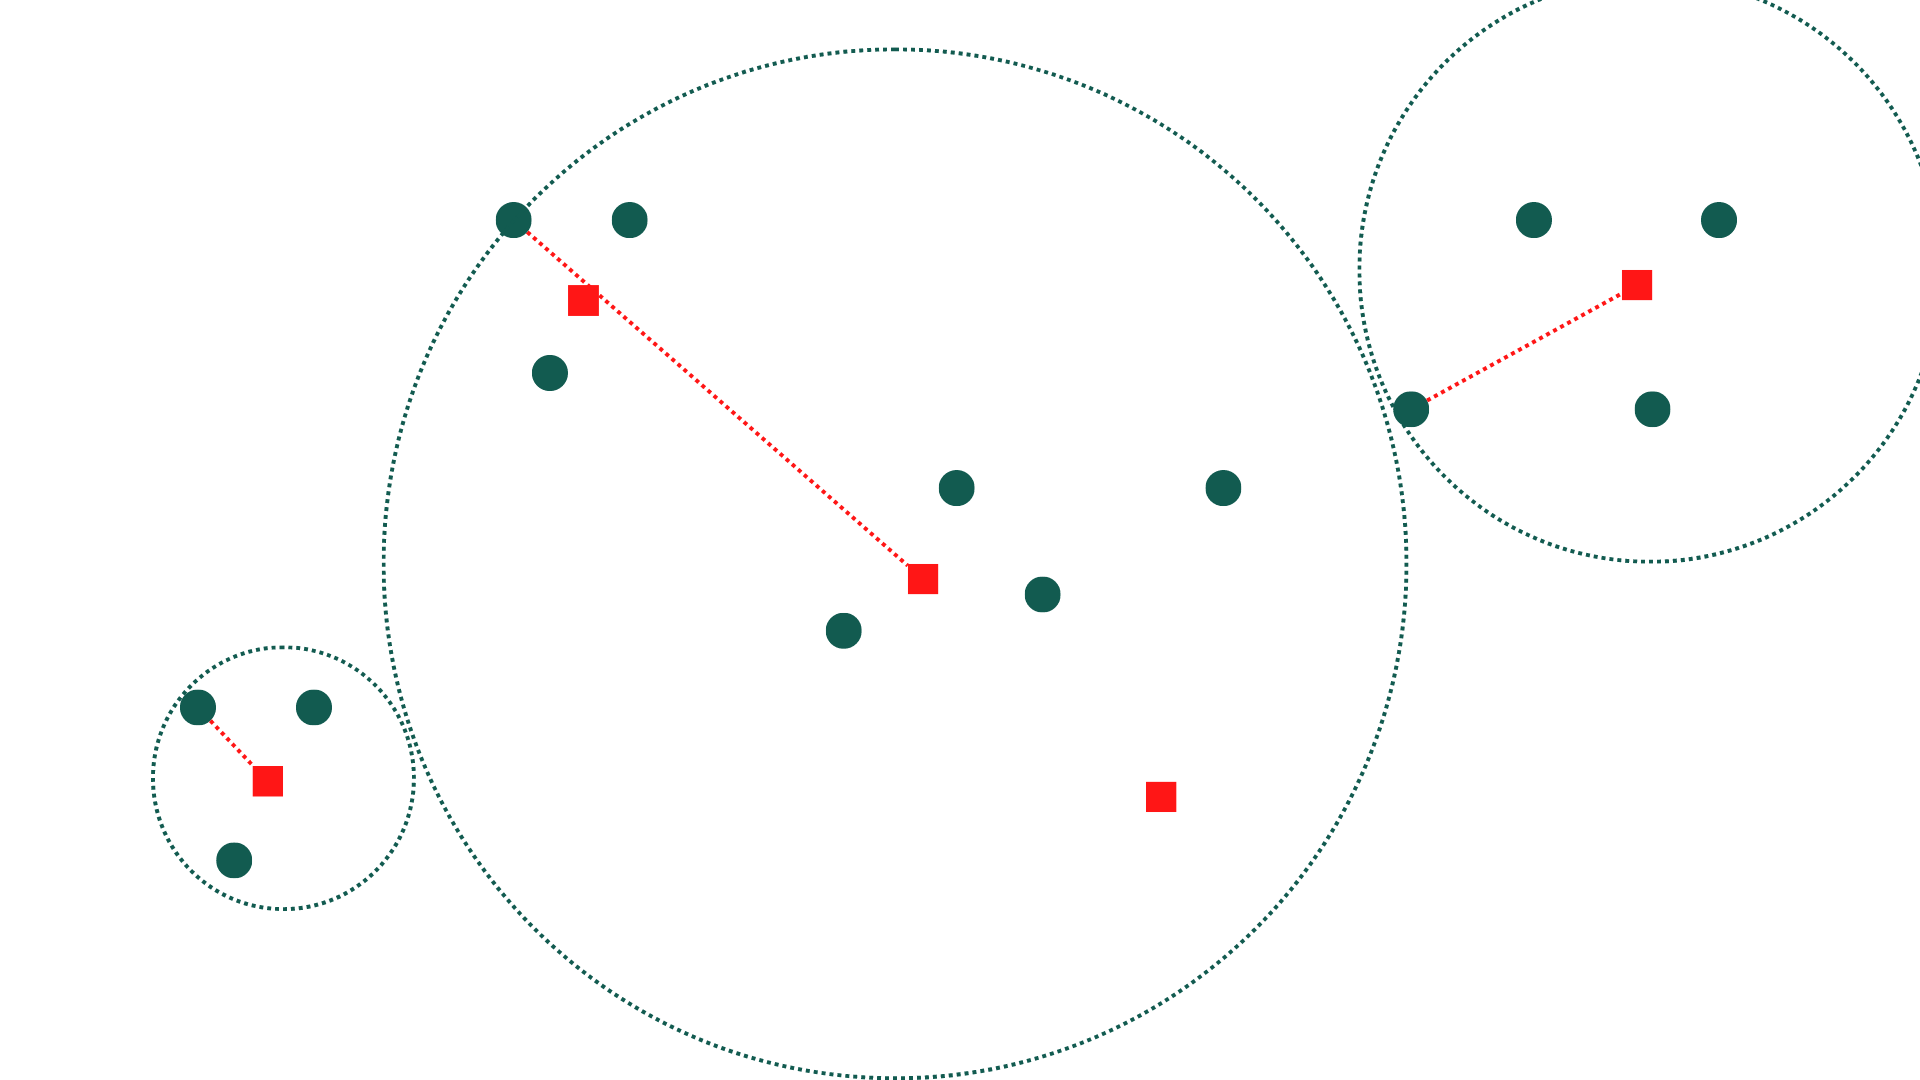
\includegraphics[width=350pt]{./10.png}
\end{frame}
   
\begin{frame}[c]
    \frametitle{Dry Run}
    \centering 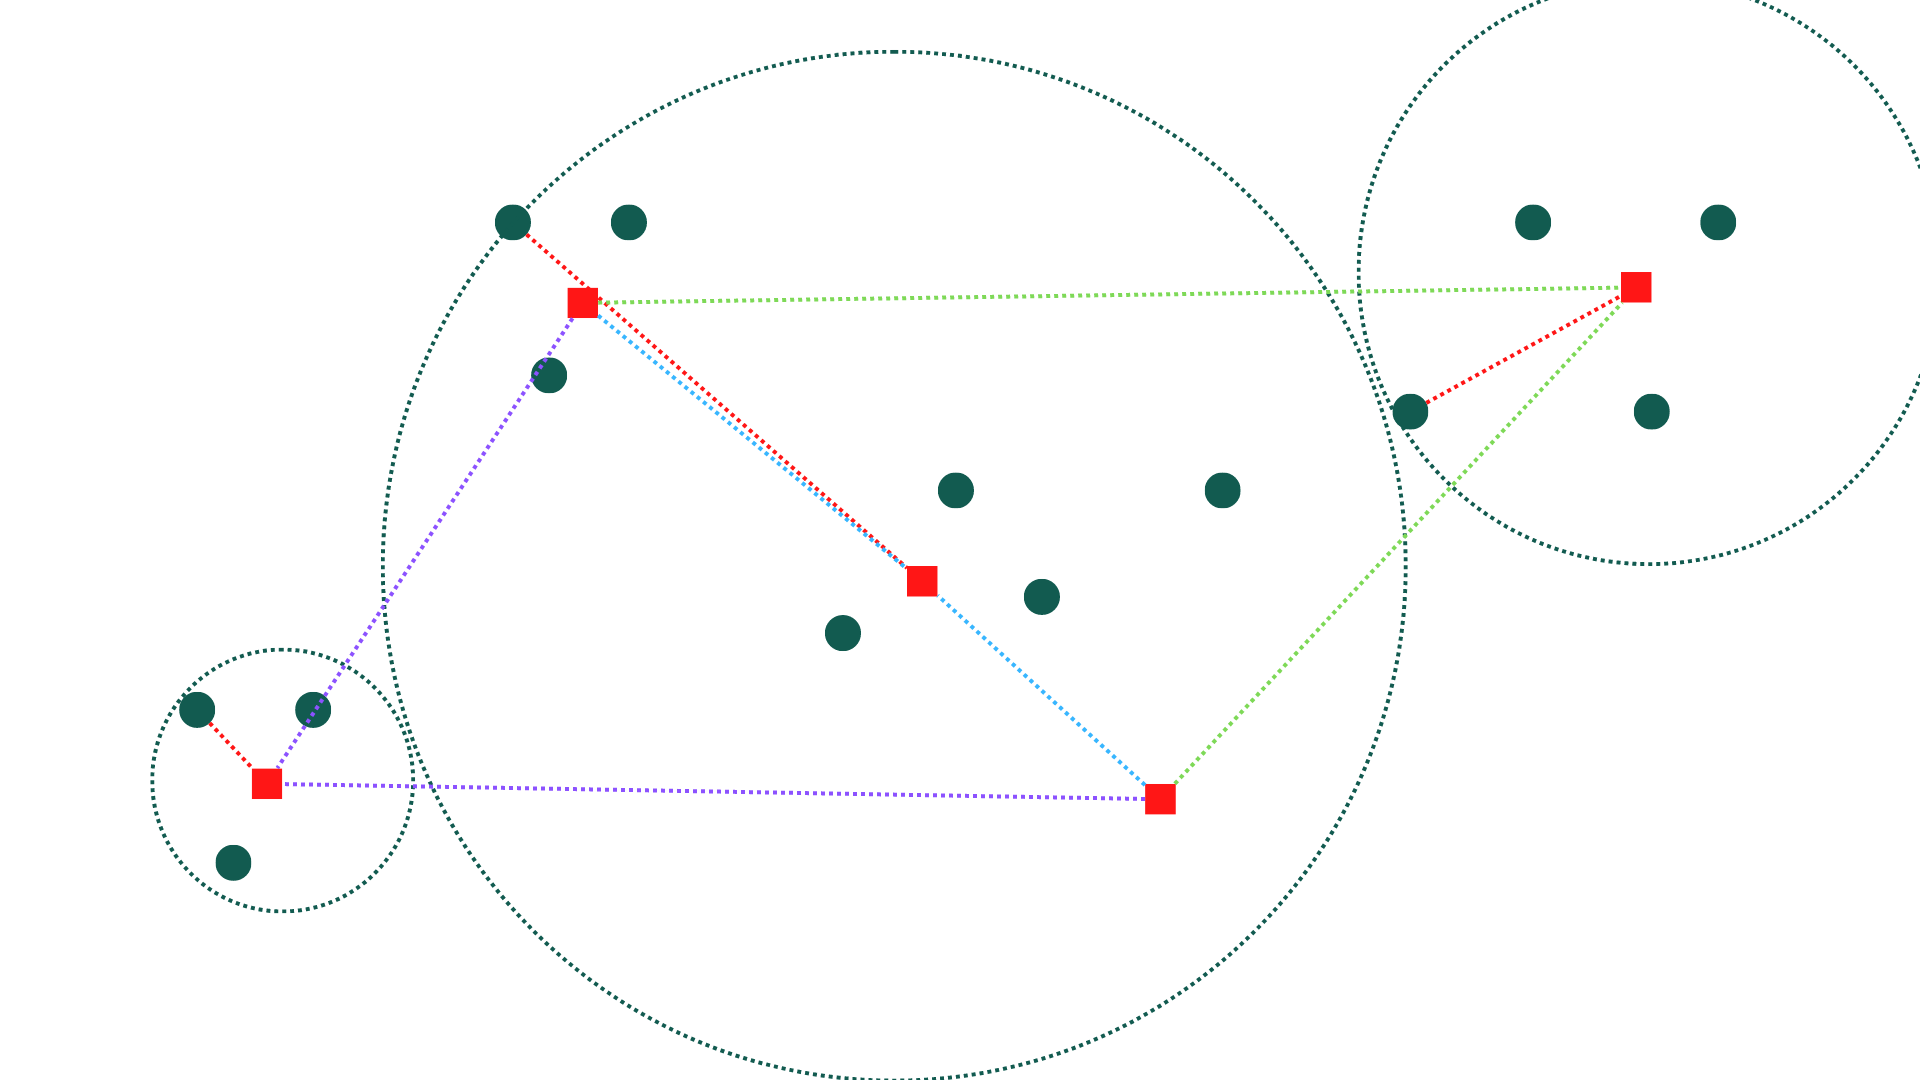
\includegraphics[width=350pt]{./11.png}
\end{frame}

\begin{frame}[c]
    \frametitle{Dry Run}
    \centering 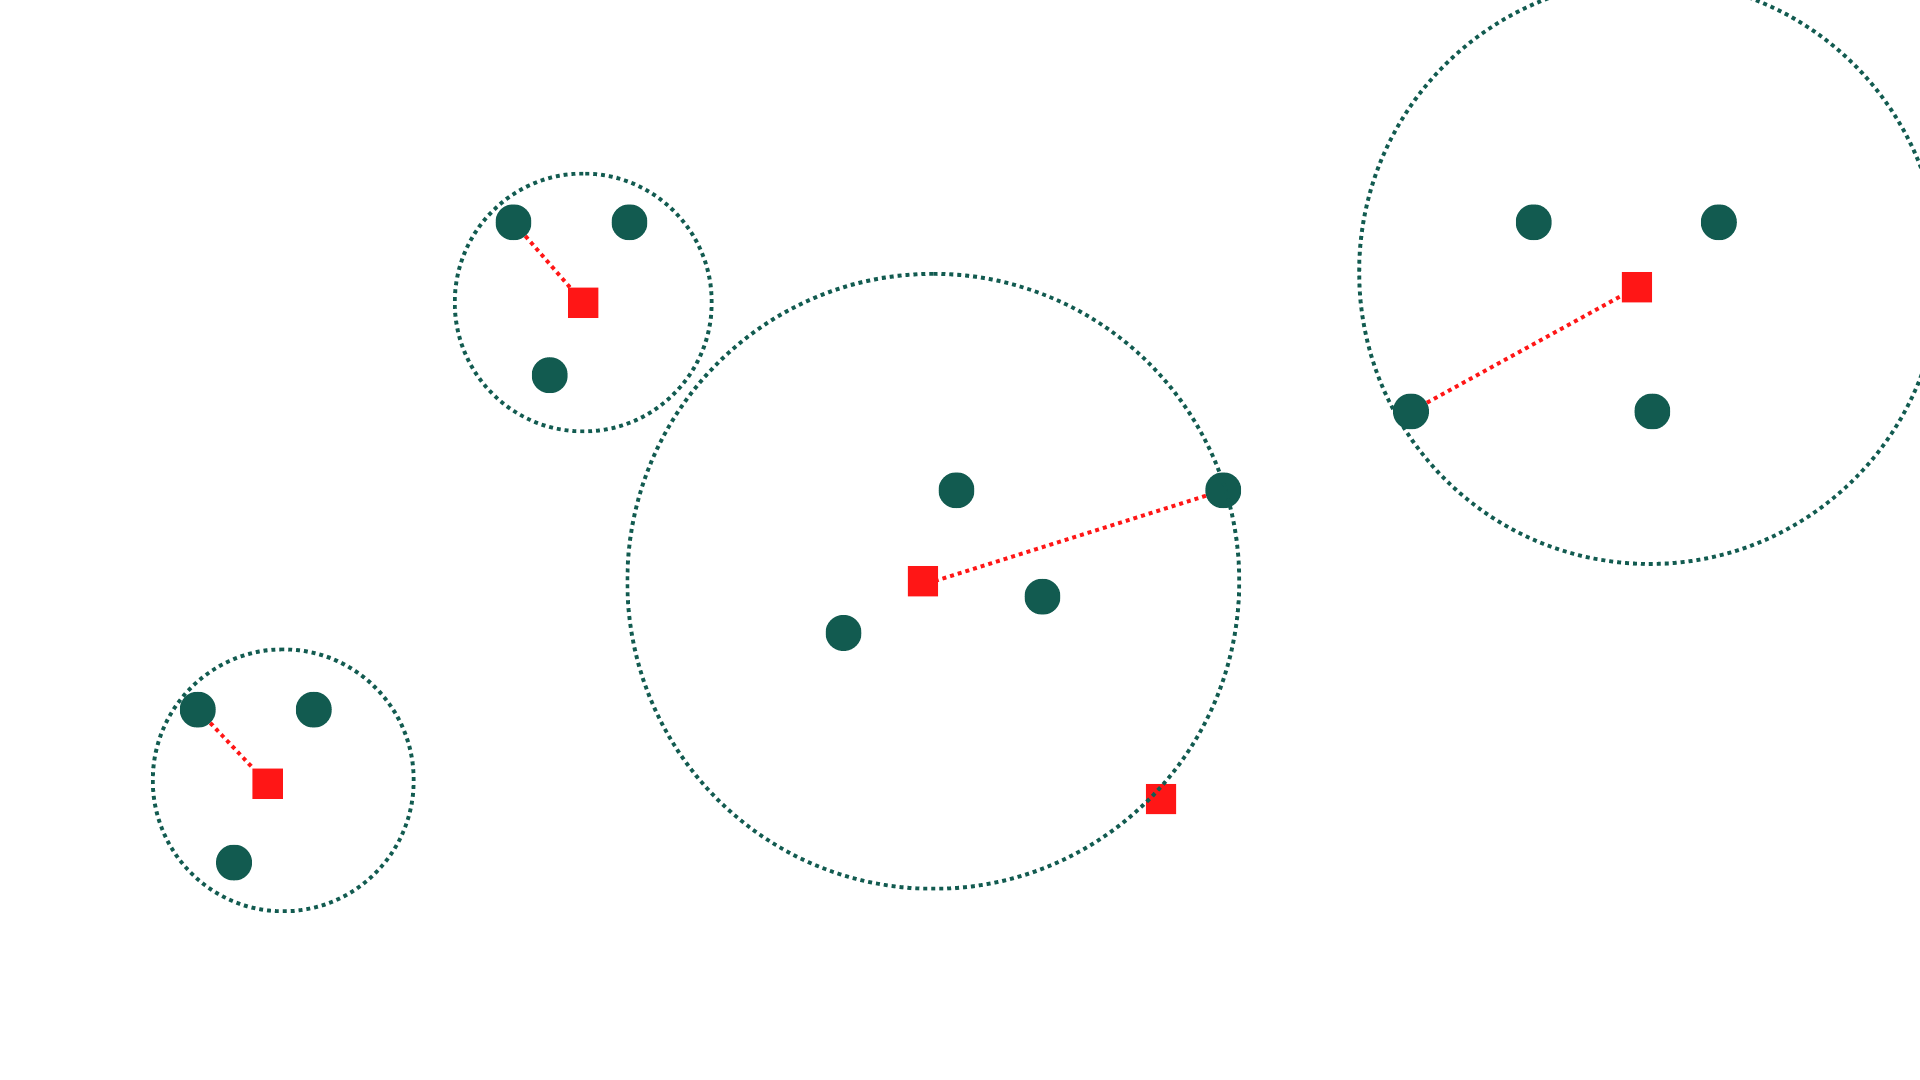
\includegraphics[width=350pt]{./12.png}
\end{frame}

\begin{frame}[c]
    \frametitle{Can We Do Better?}
    \centering 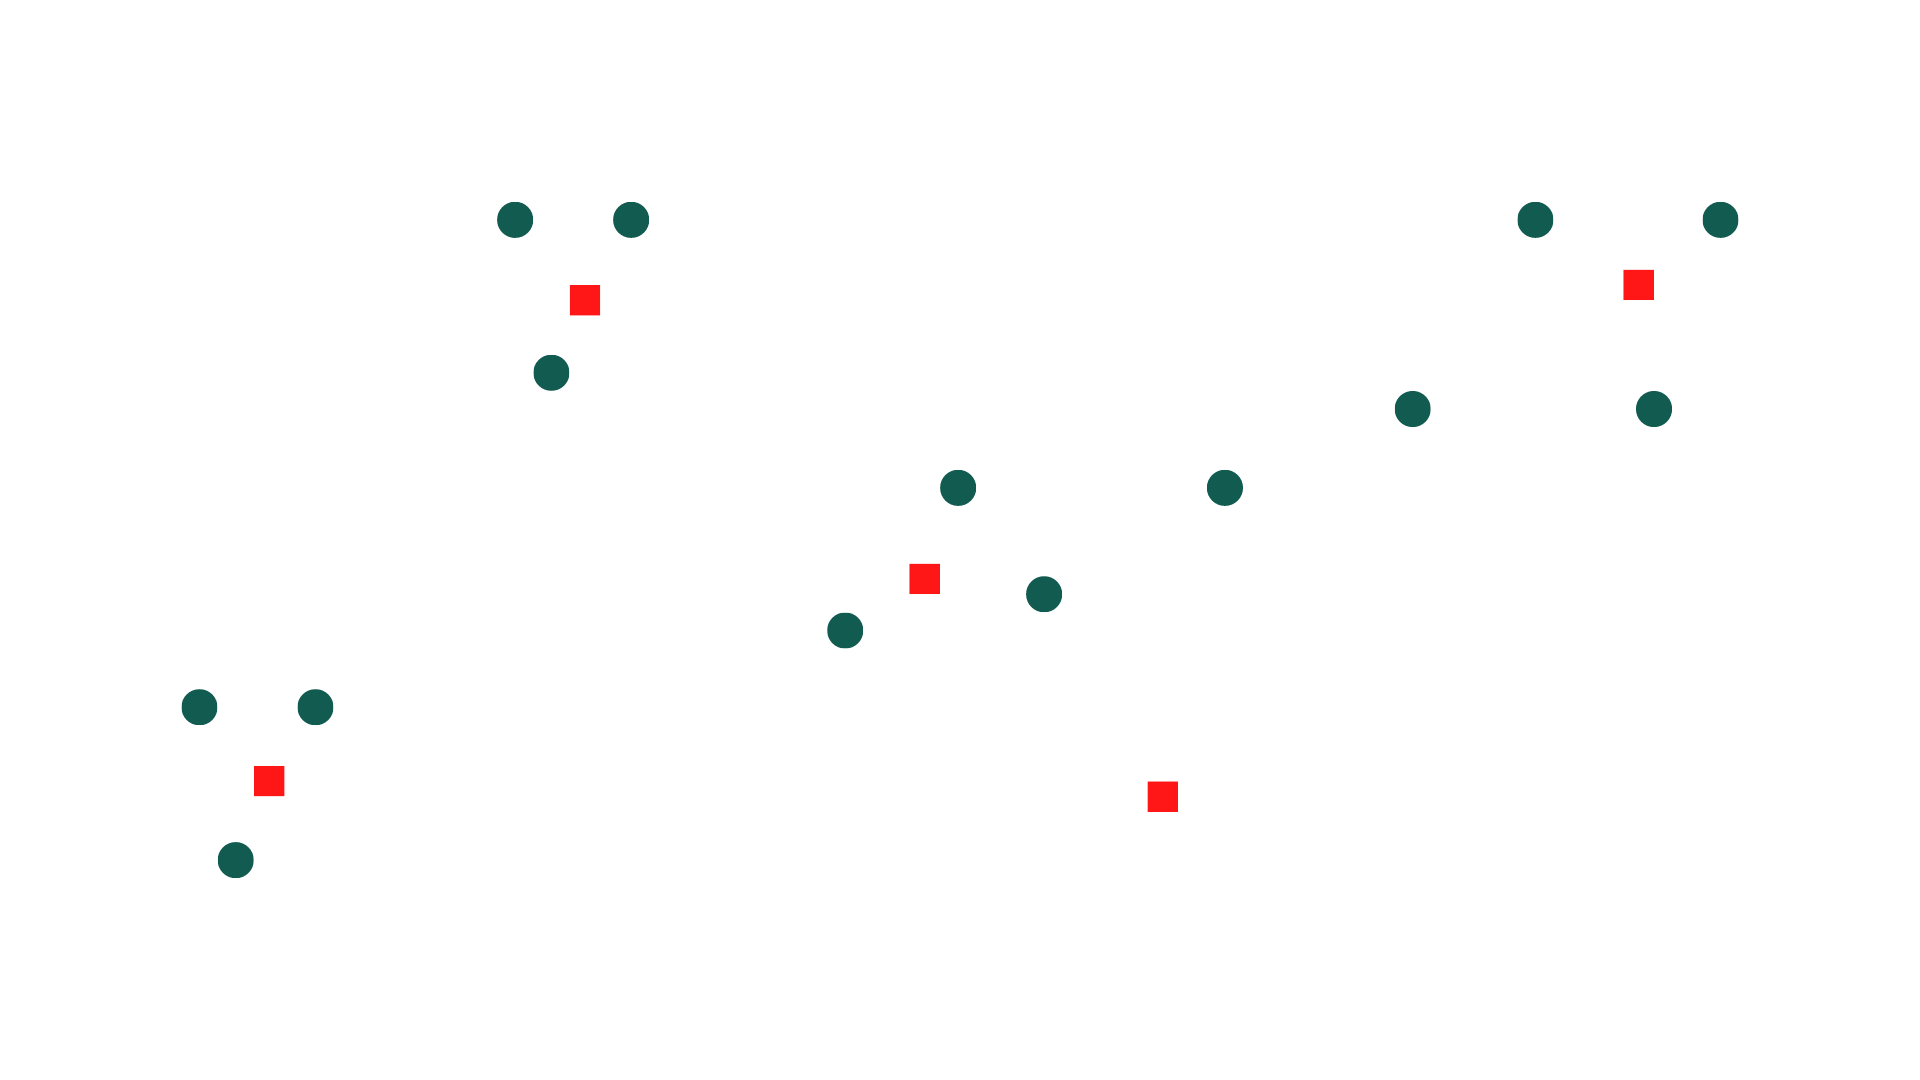
\includegraphics[width=350pt]{./5.png}
\end{frame}

\begin{frame}[c]
    \frametitle{Can We Do Better?}
    \centering 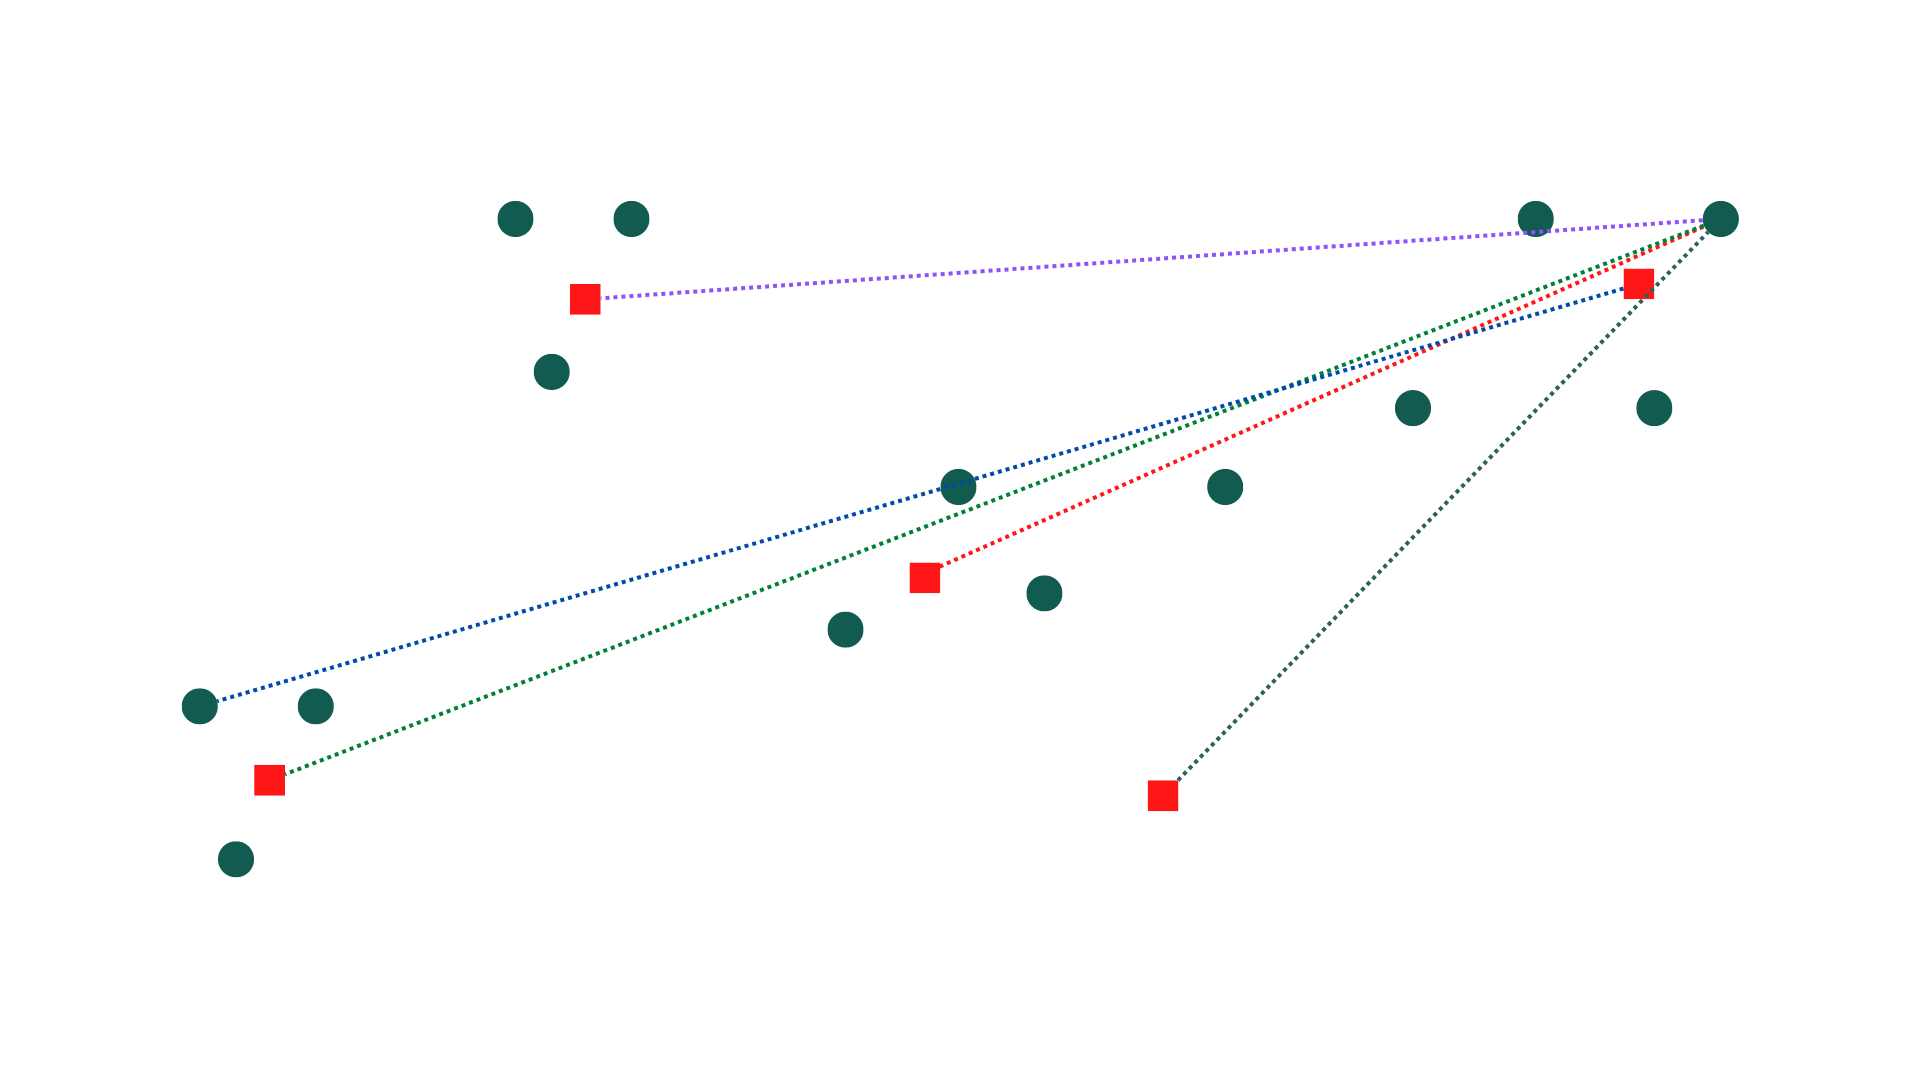
\includegraphics[width=350pt]{./13.png}
\end{frame}
   
\begin{frame}
    \frametitle{Greedy Heuristic}
    
    \begin{enumerate}
        \item Precompute distances from all users to all hospitals and record the closest hospital for each user.
        \item Select the first center. Consider the distance to the farthest user from this center as the radius to cover all the users.
        \item Select the next center from remaining hospitals such that its distance is maximum from already selected centers.
        \item Consider a subset of users for which this selected center is the closest one. Select the farthest such user. All users within that distance will now be covered by this new center.
        \item Keep the remaining users assigned to the centers they are covered by.
        \item Repeat 3-5 until $k$ hospitals have been chosen as centers.
    \end{enumerate}
\end{frame}


\begin{frame}
    \frametitle{Analysis}
        
    \begin{itemize}
        \item Time to calculate precompute distances is $O(1)$ for a connected graph -- selecting nearest or farthest node is $O(|V|)$.
        \item Time to select the first center is $O(1)$ if selected at random.
        \item Time to select the first center if we select on the basis of minimum distance to farthest user is $O(|V|^2)$.
        \item Time for selecting the farthest center from the selected centers is $O(|V|^2)$ -- iterate $(k - 1)$ times.
        \item Total Time Complexity of Greedy Heuristic is given by $O(k \cdot|V|^2)$
    \end{itemize}
\end{frame}

\begin{frame}
\frametitle {Counter Example}
\end{frame}

\begin{frame}
    \frametitle{References}
    \begin{itemize}
        \item Rana, R., Garg, D. (2009). Heuristic Approaches for K-Center Problem. 2009 IEEE International Advance Computing Conference. doi:10.1109/iadcc.2009.4809031
        \item Algorithm Design -- Kleinberg and Tardos
    \end{itemize}
\end{frame}
\end{document}
